% ============================================================
%  CHAPTER 3 — Hardware Platform
% ============================================================
\chapter{Hardware Platform}
\label{ch:hardware}

\section{PAL Robotics TIAGo}

\tiago{} (Take It And Go) is a mobile manipulator robot developed by PAL Robotics,
designed for research and service applications in domestic and industrial environments.
It combines an omnidirectional mobile base, a variable-height torso, a 7-DOF
manipulator arm, and a rich sensor suite into a single integrated platform.
Figure~\ref{fig:tiago_overview} illustrates the robot's main components.

\begin{figure}[H]
  \centering
  \includegraphics[width=0.55\textwidth]{figures/TIAGo_overview.png}
  \caption{Overview of the TIAGo mobile manipulator showing all major subsystems.
           Image courtesy of PAL Robotics.}
  \label{fig:tiago_overview}
\end{figure}

\subsection{Technical Specifications}

\begin{figure}[H]
  \centering
  \begin{minipage}{0.48\textwidth}
    \centering
    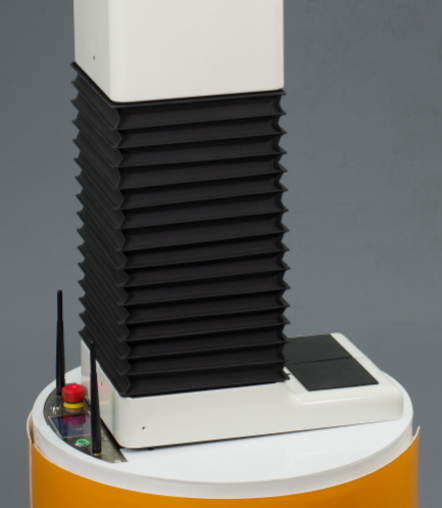
\includegraphics[width=\linewidth]{figures/Torso_lifter.png}
    \caption{TIAGo torso lift mechanism (prismatic joint, world-Z aligned).
             Image courtesy of PAL Robotics.}
    \label{fig:torso_lifter}
  \end{minipage}
  \hfill
  \begin{minipage}{0.48\textwidth}
    \centering
    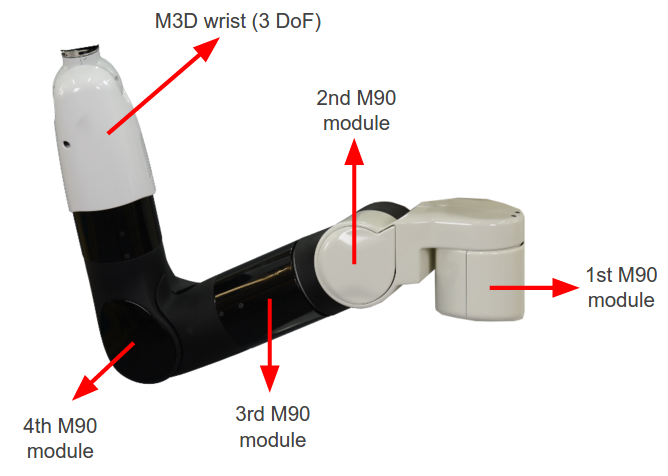
\includegraphics[width=\linewidth]{figures/Arm.png}
    \caption{TIAGo 7-DOF arm — four M90 modules and a 3-DOF wrist.
             Image courtesy of PAL Robotics.}
    \label{fig:arm_components}
  \end{minipage}
\end{figure}

Table~\ref{tab:tiago_specs} lists the key technical parameters of the \tiago{}
platform used in this work.

\begin{table}[H]
\centering
\caption{TIAGo technical specifications.}
\label{tab:tiago_specs}
\begin{tabular}{ll}
\toprule
\textbf{Parameter} & \textbf{Value} \\
\midrule
\multicolumn{2}{l}{\textit{Mobile Base}} \\
Locomotion     & Omnidirectional differential drive \\
Max speed      & 1.0 m/s \\
Payload        & 50 kg \\
Navigation     & ROS move\_base with laser odometry \\
\midrule
\multicolumn{2}{l}{\textit{Torso}} \\
Type           & Prismatic lift joint \\
Range          & 0 -- 35 cm \\
Max speed      & 3 cm/s \\
Axis           & Aligned with world Z (vertical) \\
\midrule
\multicolumn{2}{l}{\textit{Arm}} \\
DOF            & 7 \\
Joints         & Shoulder yaw, shoulder pitch, shoulder roll, \\
               & elbow, wrist yaw, wrist pitch, wrist roll \\
Reach          & $\approx$0.85 m from base\_footprint \\
Max payload    & 3 kg \\
\midrule
\multicolumn{2}{l}{\textit{Gripper}} \\
Type           & PAL parallel two-finger \\
Max opening    & 8 cm \\
Grip force     & $\approx$10 N \\
\midrule
\multicolumn{2}{l}{\textit{Head}} \\
DOF            & 2 (pan + tilt) \\
Pan range      & $\pm$1.5 rad \\
Tilt range     & $-0.8$ to $+0.4$ rad \\
Joint names    & \texttt{head\_1\_joint} (pan), \texttt{head\_2\_joint} (tilt) \\
\midrule
\multicolumn{2}{l}{\textit{Onboard Computer}} \\
CPU            & Intel Core i5 / i7 (generation varies) \\
RAM            & 16 GB \\
OS             & Ubuntu 18.04 (Docker container) \\
ROS version    & Melodic (Docker), Humble (host) \\
\bottomrule
\end{tabular}
\end{table}

\begin{figure}[H]
  \centering
  \begin{minipage}{0.48\textwidth}
    \centering
    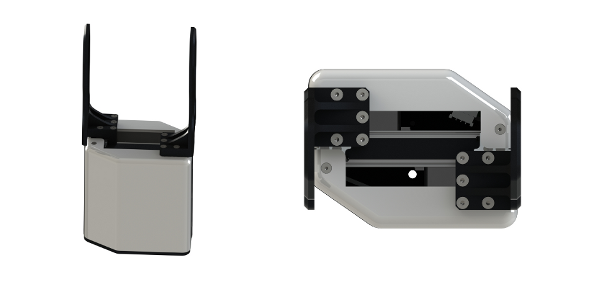
\includegraphics[width=\linewidth]{figures/Parallel_gripper.png}
    \caption{PAL parallel two-finger gripper with interchangeable fingers.
             Image courtesy of PAL Robotics.}
    \label{fig:parallel_gripper}
  \end{minipage}
  \hfill
  \begin{minipage}{0.48\textwidth}
    \centering
    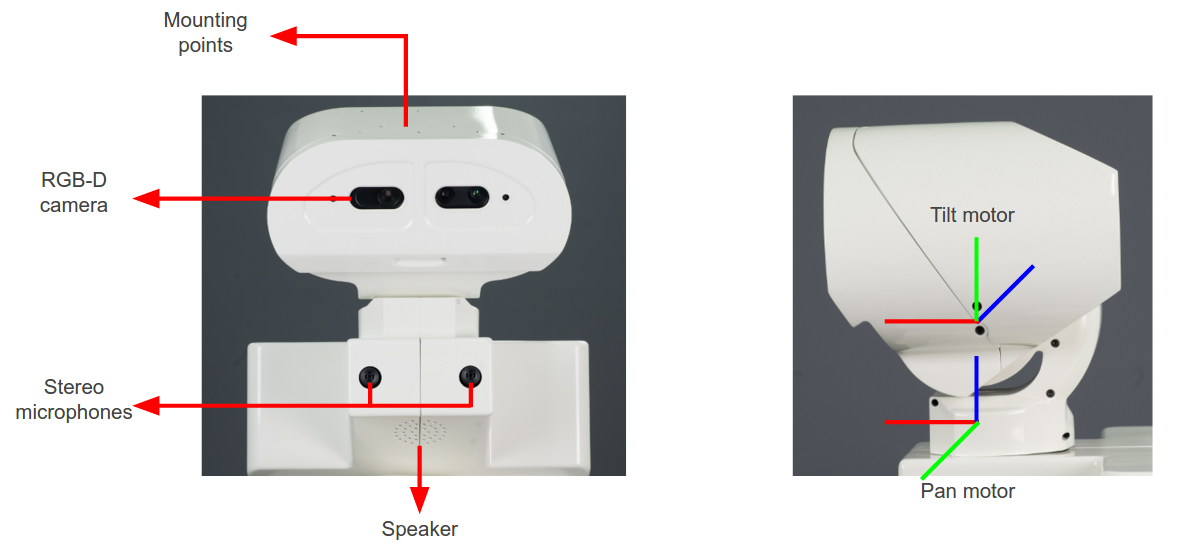
\includegraphics[width=\linewidth]{figures/Head_parts.png}
    \caption{TIAGo head assembly: pan-tilt joints, RGB-D camera, microphone
             array, and speaker. Image courtesy of PAL Robotics.}
    \label{fig:head_parts}
  \end{minipage}
\end{figure}

\section{RGB-D Sensor: Asus Xtion Pro Live}

The primary perception sensor is an \textbf{Asus Xtion Pro Live} structured-light
RGB-D camera, mounted on the robot's head.
It provides registered colour and depth images at up to 30 fps.

\begin{table}[H]
\centering
\caption{Asus Xtion Pro Live specifications.}
\label{tab:xtion_specs}
\begin{tabular}{ll}
\toprule
\textbf{Parameter} & \textbf{Value} \\
\midrule
Colour resolution  & 640 $\times$ 480 px (VGA) \\
Depth resolution   & 640 $\times$ 480 px \\
Frame rate         & 30 fps \\
Depth range        & 0.8 -- 3.5 m \\
Field of view (H)  & 58° \\
Field of view (V)  & 45° \\
Depth encoding     & 16-bit unsigned (16UC1) or 32-bit float (32FC1) \\
Depth registration & Depth aligned to RGB frame \\
ROS topics         & \texttt{/xtion/rgb/image\_raw} \\
                   & \texttt{/xtion/depth\_registered/image\_raw} \\
                   & \texttt{/xtion/rgb/camera\_info} \\
\bottomrule
\end{tabular}
\end{table}

The depth and colour images are delivered as time-synchronised pairs via
\begin{sloppypar}\noindent\texttt{message\_filters.ApproximateTimeSynchronizer}\end{sloppypar}
with a tolerance of 100\,ms.
Depth values are converted to metres: for 16UC1 encoding, divide by 1000; for 32FC1,
the values are already in metres.
Pixels with $d < 0.15$ m or $d > 3.5$ m are discarded as invalid.

\begin{figure}[H]
  \centering
  \begin{minipage}{0.48\textwidth}
    \centering
    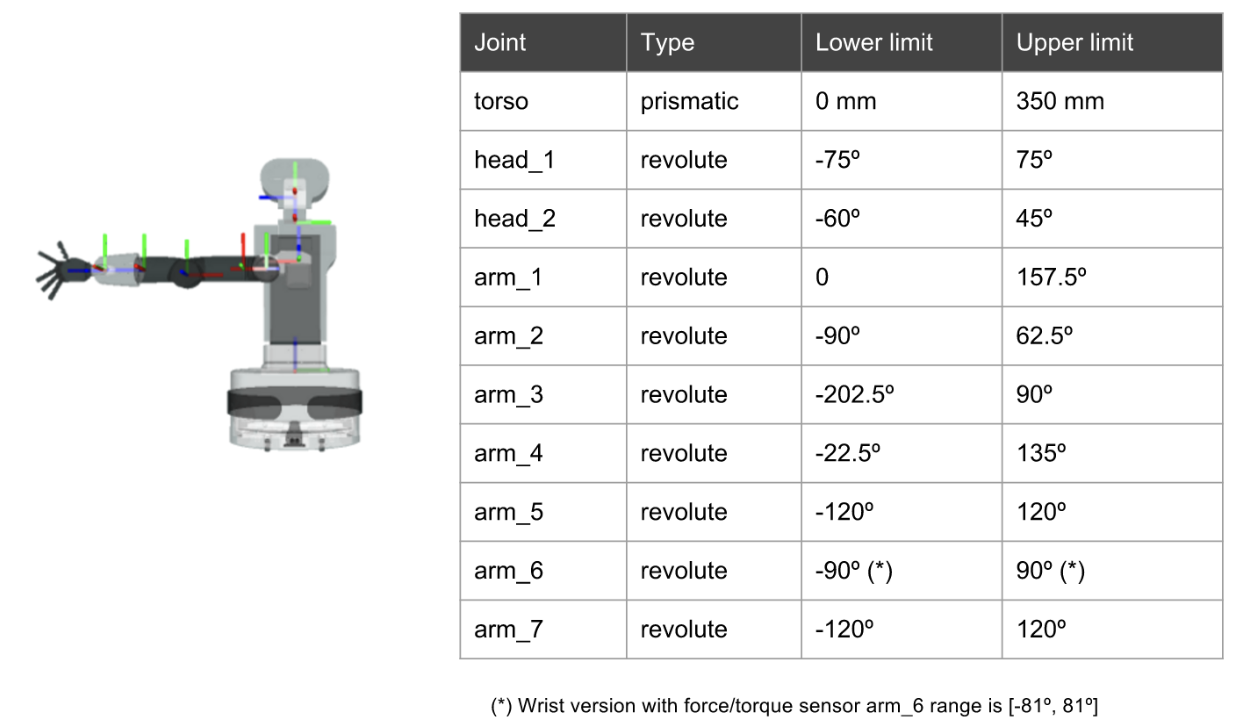
\includegraphics[width=\linewidth]{figures/kinematics.png}
    \caption{TIAGo upper-body joint kinematics and motion range.
             Image courtesy of PAL Robotics.}
    \label{fig:kinematics}
  \end{minipage}
  \hfill
  \begin{minipage}{0.48\textwidth}
    \centering
    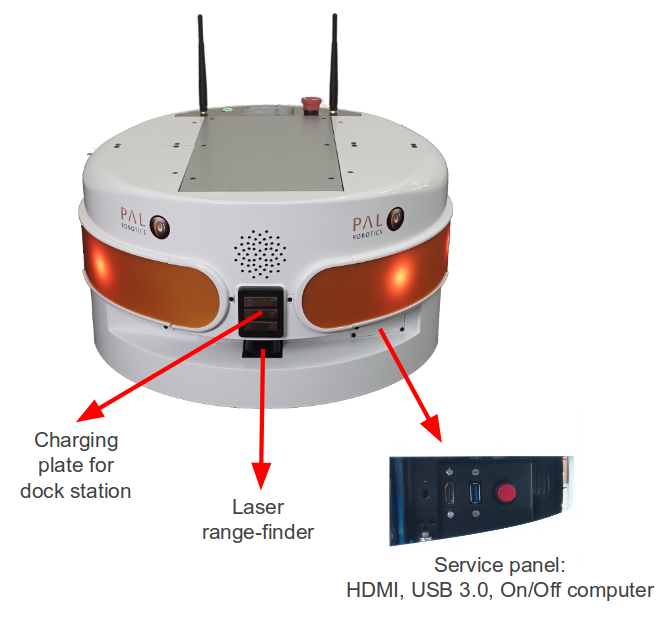
\includegraphics[width=\linewidth]{figures/Mobile_base_frontal.png}
    \caption{TIAGo omnidirectional mobile base (frontal view).
             Image courtesy of PAL Robotics.}
    \label{fig:mobile_base}
  \end{minipage}
\end{figure}

\section{Audio System}

\subsection{Microphone}

Voice input is captured via a USB audio device.
The agent scans available audio devices at startup and selects in priority order:
\begin{enumerate}[noitemsep]
  \item Devices containing ``Andrea'' or ``USB Audio'' in their name (USB microphone)
  \item Devices containing ``HDA Intel PCH: ALC'' (integrated audio)
  \item System default (fallback)
\end{enumerate}

When PulseAudio is active (detected via \texttt{PULSE\_SERVER} environment variable),
the default PulseAudio device is used unconditionally to avoid ALSA \texttt{hw:x,x}
conflicts inside the Docker container.

\subsection{Speaker / TTS}

Speech output is provided by the PAL TTS system, accessed via the
\texttt{/tts} action server (\texttt{pal\_interaction\_msgs/TtsAction}).
The language is set to British English (\texttt{en\_GB}).

\section{Deployment Environment}

\subsection{Docker Container}

All ROS-facing code runs inside a Docker container based on the PAL Robotics
software stack.
The container is named \texttt{reverent\_einstein} and runs with \texttt{--network host},
sharing the host's network namespace.

\begin{table}[H]
\centering
\caption{Docker container software environment.}
\label{tab:docker_env}
\begin{tabular}{ll}
\toprule
\textbf{Component} & \textbf{Version} \\
\midrule
Base OS            & Ubuntu 18.04 \\
Python             & 3.6 \\
ROS                & Melodic \\
OpenCV             & 3.x (from ROS) \\
NumPy              & 1.x \\
requests           & 2.x \\
speech\_recognition & 3.x \\
\bottomrule
\end{tabular}
\end{table}

\subsection{Host Machine}

The host machine runs Ubuntu 22.04 with Python 3.10, enabling the use of modern
deep learning libraries that are incompatible with Python 3.6.

\begin{table}[H]
\centering
\caption{Host machine software environment.}
\label{tab:host_env}
\begin{tabular}{ll}
\toprule
\textbf{Component} & \textbf{Version} \\
\midrule
OS                 & Ubuntu 22.04 \\
Python             & 3.10 \\
ROS                & Humble \\
Ultralytics        & 8.4.13+ \\
PyTorch            & 2.x \\
YOLO11n weights    & COCO pre-trained \\
\bottomrule
\end{tabular}
\end{table}

\subsection{Network Configuration}

The ROS master runs on the TIAGo robot at \texttt{http://10.68.0.1:11311}.
The workstation is assigned the IP \texttt{10.68.0.129}.
The environment variables \texttt{ROS\_MASTER\_URI} and \texttt{ROS\_IP} are set
accordingly inside the Docker container before launching any ROS nodes.
Since the container uses \texttt{--network host}, the YOLO service on port 5001 and
the MJPEG visualiser on port 8081 are accessible from the host browser at
\texttt{http://localhost:5001} and \texttt{http://localhost:8081} respectively.

\section{ROS Action Servers and Topics}

The system relies on the following ROS action servers being available on the robot:

\begin{table}[H]
\centering
\caption{ROS action servers used by the agent.}
\label{tab:action_servers}
\footnotesize
\begin{tabularx}{\linewidth}{lXl}
\toprule
\textbf{Action server} & \textbf{Purpose} & \textbf{Type} \\
\midrule
\texttt{/play\_motion}                               & Pre-defined arm/body motions & PlayMotionAction \\
\texttt{/move\_group}                                & MoveIt motion planning       & MoveGroupAction \\
\texttt{/tts}                                        & PAL text-to-speech           & TtsAction \\
\texttt{/head\_controller/follow\_joint\_trajectory} & Head pan/tilt control        & FollowJointTrajAction \\
\texttt{/torso\_controller/follow\_joint\_trajectory}& Torso lift control           & FollowJointTrajAction \\
\texttt{/arm\_controller/follow\_joint\_trajectory}  & Direct arm joint control     & FollowJointTrajAction \\
\texttt{/move\_base}                                 & Navigation                   & MoveBaseAction \\
\bottomrule
\end{tabularx}
\normalsize
\end{table}
